% Options for packages loaded elsewhere
\PassOptionsToPackage{unicode}{hyperref}
\PassOptionsToPackage{hyphens}{url}
%
\documentclass[
  12pt,
  oneside]{book}
\usepackage{amsmath,amssymb}
\usepackage{lmodern}
\usepackage{setspace}
\usepackage{iftex}
\ifPDFTeX
  \usepackage[T1]{fontenc}
  \usepackage[utf8]{inputenc}
  \usepackage{textcomp} % provide euro and other symbols
\else % if luatex or xetex
  \usepackage{unicode-math}
  \defaultfontfeatures{Scale=MatchLowercase}
  \defaultfontfeatures[\rmfamily]{Ligatures=TeX,Scale=1}
\fi
% Use upquote if available, for straight quotes in verbatim environments
\IfFileExists{upquote.sty}{\usepackage{upquote}}{}
\IfFileExists{microtype.sty}{% use microtype if available
  \usepackage[]{microtype}
  \UseMicrotypeSet[protrusion]{basicmath} % disable protrusion for tt fonts
}{}
\makeatletter
\@ifundefined{KOMAClassName}{% if non-KOMA class
  \IfFileExists{parskip.sty}{%
    \usepackage{parskip}
  }{% else
    \setlength{\parindent}{0pt}
    \setlength{\parskip}{6pt plus 2pt minus 1pt}}
}{% if KOMA class
  \KOMAoptions{parskip=half}}
\makeatother
\usepackage{xcolor}
\IfFileExists{xurl.sty}{\usepackage{xurl}}{} % add URL line breaks if available
\IfFileExists{bookmark.sty}{\usepackage{bookmark}}{\usepackage{hyperref}}
\hypersetup{
  hidelinks,
  pdfcreator={LaTeX via pandoc}}
\urlstyle{same} % disable monospaced font for URLs
\usepackage[a4paper, left=3.5cm, right=2.5cm, top=2.5cm, bottom=2.5cm]{geometry}
\usepackage{color}
\usepackage{fancyvrb}
\newcommand{\VerbBar}{|}
\newcommand{\VERB}{\Verb[commandchars=\\\{\}]}
\DefineVerbatimEnvironment{Highlighting}{Verbatim}{commandchars=\\\{\}}
% Add ',fontsize=\small' for more characters per line
\usepackage{framed}
\definecolor{shadecolor}{RGB}{248,248,248}
\newenvironment{Shaded}{\begin{snugshade}}{\end{snugshade}}
\newcommand{\AlertTok}[1]{\textcolor[rgb]{0.94,0.16,0.16}{#1}}
\newcommand{\AnnotationTok}[1]{\textcolor[rgb]{0.56,0.35,0.01}{\textbf{\textit{#1}}}}
\newcommand{\AttributeTok}[1]{\textcolor[rgb]{0.77,0.63,0.00}{#1}}
\newcommand{\BaseNTok}[1]{\textcolor[rgb]{0.00,0.00,0.81}{#1}}
\newcommand{\BuiltInTok}[1]{#1}
\newcommand{\CharTok}[1]{\textcolor[rgb]{0.31,0.60,0.02}{#1}}
\newcommand{\CommentTok}[1]{\textcolor[rgb]{0.56,0.35,0.01}{\textit{#1}}}
\newcommand{\CommentVarTok}[1]{\textcolor[rgb]{0.56,0.35,0.01}{\textbf{\textit{#1}}}}
\newcommand{\ConstantTok}[1]{\textcolor[rgb]{0.00,0.00,0.00}{#1}}
\newcommand{\ControlFlowTok}[1]{\textcolor[rgb]{0.13,0.29,0.53}{\textbf{#1}}}
\newcommand{\DataTypeTok}[1]{\textcolor[rgb]{0.13,0.29,0.53}{#1}}
\newcommand{\DecValTok}[1]{\textcolor[rgb]{0.00,0.00,0.81}{#1}}
\newcommand{\DocumentationTok}[1]{\textcolor[rgb]{0.56,0.35,0.01}{\textbf{\textit{#1}}}}
\newcommand{\ErrorTok}[1]{\textcolor[rgb]{0.64,0.00,0.00}{\textbf{#1}}}
\newcommand{\ExtensionTok}[1]{#1}
\newcommand{\FloatTok}[1]{\textcolor[rgb]{0.00,0.00,0.81}{#1}}
\newcommand{\FunctionTok}[1]{\textcolor[rgb]{0.00,0.00,0.00}{#1}}
\newcommand{\ImportTok}[1]{#1}
\newcommand{\InformationTok}[1]{\textcolor[rgb]{0.56,0.35,0.01}{\textbf{\textit{#1}}}}
\newcommand{\KeywordTok}[1]{\textcolor[rgb]{0.13,0.29,0.53}{\textbf{#1}}}
\newcommand{\NormalTok}[1]{#1}
\newcommand{\OperatorTok}[1]{\textcolor[rgb]{0.81,0.36,0.00}{\textbf{#1}}}
\newcommand{\OtherTok}[1]{\textcolor[rgb]{0.56,0.35,0.01}{#1}}
\newcommand{\PreprocessorTok}[1]{\textcolor[rgb]{0.56,0.35,0.01}{\textit{#1}}}
\newcommand{\RegionMarkerTok}[1]{#1}
\newcommand{\SpecialCharTok}[1]{\textcolor[rgb]{0.00,0.00,0.00}{#1}}
\newcommand{\SpecialStringTok}[1]{\textcolor[rgb]{0.31,0.60,0.02}{#1}}
\newcommand{\StringTok}[1]{\textcolor[rgb]{0.31,0.60,0.02}{#1}}
\newcommand{\VariableTok}[1]{\textcolor[rgb]{0.00,0.00,0.00}{#1}}
\newcommand{\VerbatimStringTok}[1]{\textcolor[rgb]{0.31,0.60,0.02}{#1}}
\newcommand{\WarningTok}[1]{\textcolor[rgb]{0.56,0.35,0.01}{\textbf{\textit{#1}}}}
\usepackage{longtable,booktabs,array}
\usepackage{calc} % for calculating minipage widths
% Correct order of tables after \paragraph or \subparagraph
\usepackage{etoolbox}
\makeatletter
\patchcmd\longtable{\par}{\if@noskipsec\mbox{}\fi\par}{}{}
\makeatother
% Allow footnotes in longtable head/foot
\IfFileExists{footnotehyper.sty}{\usepackage{footnotehyper}}{\usepackage{footnote}}
\makesavenoteenv{longtable}
\usepackage{graphicx}
\makeatletter
\def\maxwidth{\ifdim\Gin@nat@width>\linewidth\linewidth\else\Gin@nat@width\fi}
\def\maxheight{\ifdim\Gin@nat@height>\textheight\textheight\else\Gin@nat@height\fi}
\makeatother
% Scale images if necessary, so that they will not overflow the page
% margins by default, and it is still possible to overwrite the defaults
% using explicit options in \includegraphics[width, height, ...]{}
\setkeys{Gin}{width=\maxwidth,height=\maxheight,keepaspectratio}
% Set default figure placement to htbp
\makeatletter
\def\fps@figure{htbp}
\makeatother
\setlength{\emergencystretch}{3em} % prevent overfull lines
\providecommand{\tightlist}{%
  \setlength{\itemsep}{0pt}\setlength{\parskip}{0pt}}
\setcounter{secnumdepth}{5}
%%% Packages and options
\usepackage[none]{hyphenat}
\usepackage{tocbibind}
\usepackage{hyperref}
\usepackage{setspace}
\raggedbottom
\usepackage{ctable}
\usepackage[T1]{fontenc}
\usepackage[utf8]{inputenc}
\usepackage{pdflscape}
\usepackage{pdfpages}
\usepackage{xspace}
\usepackage[english]{babel}
\usepackage{listings}
\usepackage{amsmath}
\usepackage{amssymb}
\usepackage{xcolor}
\usepackage{float}

%%% Force inclusion of fonts (missing ligatures from embedded pdfs)
\pdfinclusioncopyfonts=1

%%% Fonts
% Microtype setup
\microtypesetup{activate = {true, nocompatibility}, final, tracking = true, kerning = true, spacing = true, factor = 1100, stretch = 10, shrink = 10}
\SetProtrusion{encoding={*},family={bch},series={*},size={6,7}}
              {1={ ,750},2={ ,500},3={ ,500},4={ ,500},5={ ,500},
               6={ ,500},7={ ,600},8={ ,500},9={ ,500},0={ ,500}}
\SetExtraKerning[unit=space]
    {encoding={*}, family={bch}, series={*}, size={footnotesize,small,normalsize}}
    {\textendash={400,400}, % en-dash, add more space around it
     "28={ ,150}, % left bracket, add space from right
     "29={150, }, % right bracket, add space from left
     \textquotedblleft={ ,150}, % left quotation mark, space from right
     \textquotedblright={150, }} % right quotation mark, space from left
\SetExtraKerning[unit=space]
   {encoding={*}, family={qhv}, series={b}, size={large,Large}}
   {1={-200,-200},
    \textendash={400,400}}
\SetTracking{encoding={*}, shape=sc}{40}
\microtypecontext{spacing=nonfrench}

% Body and maths
% I used libertinus and libertinus math, uncomment the next lines to use
% \usepackage[sb, osf]{libertinus}
% \usepackage{libertinust1math}

% Monospace font for code listings
% I used Inconsolata, uncomment the next line to use
% \usepackage[narrow, scaled = 0.95, mono]{inconsolata}

%%% Define new environment for dedication
\newenvironment{dedication}
  {\thispagestyle{empty}
   \vspace*{\stretch{1}}
   \raggedleft
  }
  {\par
   \vspace{\stretch{3}}
   \cleardoublepage
  }

%%% Change size of figures' captions
% \usepackage[font = small, labelfont = sc]{caption}

%%% New command for defining vectors
\usepackage{bm}
\newcommand{\vect}[1]{\boldsymbol{\mathbf{#1}}}

%%% New command for adding ^st, ^nd, ^rd, ^th
\newcommand{\first}[0]{\(1\)\textsuperscript{st}}
\newcommand{\second}[0]{\(2\)\textsuperscript{nd}}
\newcommand{\third}[0]{\(3\)\textsuperscript{rd}}
\newcommand{\ith}[1]{\(#1\)\textsuperscript{th}}

%%% Variance command
\newcommand{\Var}[0]{\text{Var}}
\newcommand{\var}[0]{\text{var}}
\newcommand{\Cov}[0]{\text{Cov}}
\newcommand{\cov}[0]{\text{cov}}
\newcommand{\Corr}[0]{\text{Corr}}
\newcommand{\corr}[0]{\text{corr}}

%%% New command for n_obs and n_sim
\newcommand{\nobs}[0]{n_{\text{obs}}}
\newcommand{\nsims}[0]{n_{\text{sim}}}

%%% New command for logit function
\newcommand{\logit}{\text{logit}}

%%% hyperref setup
% pdf meta-data goes here
% \hypersetup{pdfauthor = {Name Surname},
%             pdftitle = {Title}}
% The next line will colour each link in the document
% Can be useful while writing, remove in the final version
\hypersetup{
  colorlinks = true}

%%% fancyhdr
\usepackage{fancyhdr}
\pagestyle{plain}

%%% Sort and compress references
\usepackage[sort&compress]{natbib}

%%% Customise Chapter, Section, and Subsection headers
% Uncomment to customise titles of chapters and sections
% \usepackage{titlesec}
% \titleformat{\chapter}[hang]{\LARGE\itshape\filleft}{\thechapter}{1em}{}
% \titleformat{\section}[hang]{\Large\scshape}{\thesection}{1em}{}
% \titleformat{\subsection}[hang]{\large\itshape}{\thesubsection}{1em}{}
% \titleformat{\subsubsection}[hang]{\itshape}{\thesubsubsection}{1em}{}
\ifLuaTeX
  \usepackage{selnolig}  % disable illegal ligatures
\fi
\usepackage[]{natbib}
\bibliographystyle{unsrt}

\author{}
\date{\vspace{-2.5em}}

\begin{document}

%!TEX root = YEAR-SURNAME-N-PhD.tex

\begin{titlepage}
	\begin{center}
		\doublespacing
		\vspace*{3em}
		{	\Huge
			Title \par
		}
		\vspace*{0.5em}
		\textit{by} \par
		\vspace*{0.5em}
		{	\LARGE
			Name Surname \par
		}
		\vfill
		\textsc{Department of Health Sciences} \par
		\textsc{University of Leicester} \par
		\vspace*{1.5em}
		\textsc{Thesis submitted for the degree of} \par
		\textsc{Doctor} \textit{of} \textsc{Philosophy} \par
		\vspace*{1.5em}
		{	\Large
			\textsc{Year}
		}
	\end{center}
\end{titlepage}


\pagenumbering{gobble}

\chapter*{}
\begin{dedication}
	\parbox{0.5\textwidth}{\itshape I like big quotes and I cannot lie.} \par
	\vspace*{1em}
	{	\large\scshape
		-- Anonymous \par
	}
\end{dedication}

\frontmatter

\chapter*{Abstract}
\phantomsection
\addcontentsline{toc}{chapter}{Abstract}

\begin{center}

{\LARGE Title}

% {\LARGE Title Second Line}

{\itshape by}

{\Large Name Surname}

\end{center}

\vspace*{2em}

Abstract goes here.

Bacon ipsum dolor amet pancetta chicken andouille hamburger.
Sed ad nulla ball tip hamburger fugiat salami.
Chislic tempor labore velit, officia ham hock ut mollit picanha.
Pig reprehenderit turducken id spare ribs.

Doner minim pork chop pariatur et duis ham hock tempor exercitation eiusmod sirloin mollit landjaeger.
Nisi commodo pork in spare ribs meatloaf, fugiat duis biltong picanha eu.
Duis nostrud sunt pork non irure.
Sorry Micki.
In biltong pork lorem tempor landjaeger.

In pork belly shoulder nisi tail aliqua andouille consequat anim reprehenderit pastrami.
Prosciutto sint consequat, labore salami exercitation do.
Andouille shankle nisi, deserunt adipisicing ut ex.
Laborum nulla fugiat drumstick cow venison fatback burgdoggen ham pork jowl frankfurter.
Meatloaf ullamco consectetur tongue alcatra leberkas short loin sint.
Tempor shankle tenderloin cupidatat, ex sint reprehenderit kielbasa.

\cleardoublepage

\chapter*{Acknowledgements}
\phantomsection
\addcontentsline{toc}{chapter}{Acknowledgements}

\setstretch{1.5}

Acknowledgements go here.
Don't forget to thank \emph{3.06} for the banter.

\setstretch{1.0}

\cleardoublepage

\microtypesetup{protrusion=false}

\renewcommand{\contentsname}{Table of Contents}
\tableofcontents

\listoffigures

\listoftables

\microtypesetup{protrusion=true}

\cleardoublepage

\setstretch{1.5}
\mainmatter

\hypertarget{intro}{%
\chapter{Introduction}\label{intro}}

Start by double-clicking \texttt{uol-thesis-bookdown.Rproj}.
If your RStudio is configured correctly (and you have a \LaTeX{} distribution on your machine) you should not have any issue.

You should also see a \emph{Build} tab in the RStudio UI.
Click it and then click the \emph{Build Book} button to compile the document.
Debugging issues can be weird, check \href{https://www.goodreads.com/en/book/show/29437996-copying-and-pasting-from-stack-overflow}{this book} for help with debugging in general.

Most customisations can be modified in the \texttt{latex/preamble.tex} file; however, there is a lot more that could be changed.
If you need help, open an issue on \href{https://github.com/ellessenne/uol-thesis}{this GitHub repository} and mention \texttt{bookdown}.

\hypertarget{intro-section}{%
\section{Section}\label{intro-section}}

This thesis template follows the guidelines from the University of Leicester for PhD theses.

This document uses \texttt{bookdown} (which I recommend over plain \LaTeX{}, even if you do not use R).

\begin{quote}
``Plain \LaTeX{} is just so unnecessarily complicated, make your life easier and use \texttt{bookdown}!''

-- Alessandro Gasparini
\end{quote}

Check out the \href{https://bookdown.org/yihui/bookdown/}{\texttt{bookdown} book} and the \href{https://bookdown.org/yihui/rmarkdown/}{\texttt{rmarkdown} book} for more details.

\hypertarget{methods}{%
\chapter{Methods}\label{methods}}

\hypertarget{methods-section}{%
\section{Section}\label{methods-section}}

You have syntax to link to pretty much anything in this document, see for instance Chapter \ref{intro} and Section \ref{methods-references}.

\hypertarget{methods-references}{%
\section{References}\label{methods-references}}

You can cite papers \citep{gasparini_2018}, books \citep{brent_1973}, and even combine multiple citations \citep{R, scopus}.

\hypertarget{results}{%
\chapter{Results}\label{results}}

We have a plot in Figure \ref{fig:plot} and more results in Table \ref{tab:table}.

\begin{figure}

{\centering 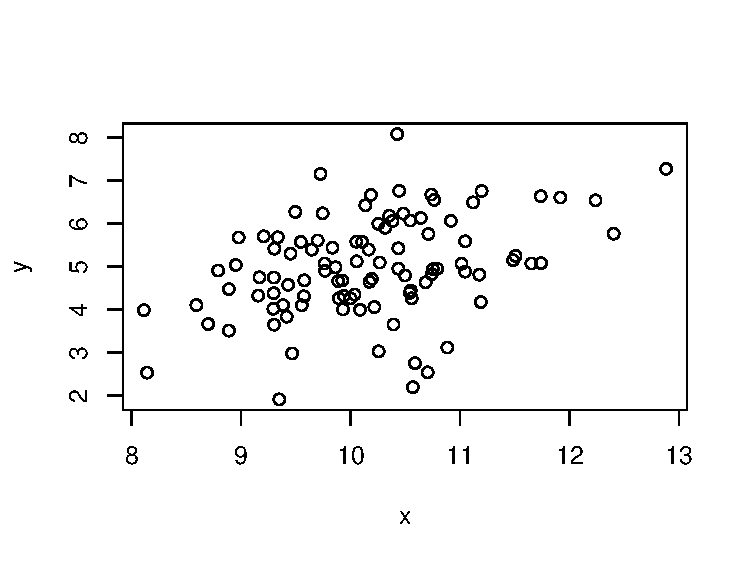
\includegraphics[width=0.8\textwidth]{YEAR-SURNAME-N-PhD_files/figure-latex/plot-1} 

}

\caption{Here goes a caption for this super-cool figure.}\label{fig:plot}
\end{figure}

\begin{table}

\caption{\label{tab:table}Caption of the table.}
\centering
\begin{tabular}[t]{rr}
\toprule
x & y\\
\midrule
10.497248 & 4.796485\\
9.301475 & 3.650826\\
9.545996 & 5.576487\\
10.686333 & 4.637482\\
10.426642 & 8.084386\\
10.086181 & 3.999149\\
\bottomrule
\end{tabular}
\end{table}

We can also include plain R output by setting the chunk option \texttt{echo\ =\ TRUE}:

\begin{Shaded}
\begin{Highlighting}[]
\NormalTok{fit }\OtherTok{\textless{}{-}} \FunctionTok{lm}\NormalTok{(y }\SpecialCharTok{\textasciitilde{}}\NormalTok{ x, }\AttributeTok{data =}\NormalTok{ tab)}
\FunctionTok{summary}\NormalTok{(fit)}
\end{Highlighting}
\end{Shaded}

\begin{verbatim}
# 
# Call:
# lm(formula = y ~ x, data = tab)
# 
# Residuals:
#      Min       1Q   Median       3Q      Max 
# -3.00075 -0.59560 -0.03597  0.83827  2.95916 
# 
# Coefficients:
#             Estimate Std. Error t value Pr(>|t|)    
# (Intercept) -0.07645    1.24382  -0.061    0.951    
# x            0.49888    0.12189   4.093 8.75e-05 ***
# ---
# Signif. codes:  0 '***' 0.001 '**' 0.01 '*' 0.05 '.' 0.1 ' ' 1
# 
# Residual standard error: 1.074 on 98 degrees of freedom
# Multiple R-squared:  0.146,   Adjusted R-squared:  0.1373 
# F-statistic: 16.75 on 1 and 98 DF,  p-value: 8.754e-05
\end{verbatim}

And more chunks:

\begin{Shaded}
\begin{Highlighting}[]
\FunctionTok{plot}\NormalTok{(fit, }\AttributeTok{which =} \DecValTok{4}\NormalTok{)}
\end{Highlighting}
\end{Shaded}

\begin{center}\includegraphics[width=0.8\textwidth]{YEAR-SURNAME-N-PhD_files/figure-latex/more-code-1} \end{center}

Note that since here we did not set the \texttt{fig.cap} chunk option, the plot did not float.

\hypertarget{discussion}{%
\chapter{Discussion}\label{discussion}}

Here goes a discussion.
Remember to talk about future work, and be confident!

\hypertarget{appendix-appendix}{%
\appendix}


\hypertarget{a-appendix}{%
\chapter{Appendix}\label{a-appendix}}

This is an appendix.
You can have extra code, published papers (if not protected by copyright), or any other supplementary information.

  \bibliography{bibliography/articles.bib,bibliography/books.bib,bibliography/others.bib}

\end{document}
